\documentclass[10pt]{beamer}

\usetheme{Frankfurt}
\useoutertheme{default}
\setbeamertemplate{footline}[page number]
\setbeamertemplate{navigation symbols}{} 

\usepackage{cmap}					% поиск в PDF
\usepackage[T2A]{fontenc}			% кодировка
\usepackage[utf8]{inputenc}			% кодировка исходного текста
\usepackage[english,russian]{babel}	% локализация и переносы
\usepackage{indentfirst}
\frenchspacing

\newcommand{\delayV}[1]{\overset{\leftarrow}{\textbf{x}}_{#1}}

\theoremstyle{definition}
\newtheorem*{Def}{Определение}

\title{Hyena Hierarchy: Towards Larger Convolutional Language Models}
\author{Крейнин Матвей}

\institute[MIPT]{Московский физико-технический институт \\ Кафедра интеллектуальных систем}

\date[2025]{}

\begin{document}
	
\begin{frame}[c]
	\titlepage
\end{frame}
	
\begin{frame}{Постановка задачи}
Дан вход $x \in \mathbb{R}^{L \times d}$ - последовательность длиной L, скрытое пространство d.

Требуется вычислить представление $y = f(x)$, которое сможет улавливать все зависимости, и ещё хорошо, если работает за:
\begin{equation*}
    \text{cost}_{time}, \text{cost}_{mem} \ll \mathbb{O}(L^2d)
\end{equation*}

Attention:
\begin{equation*}
    A(x) = \text{softmax}(\frac{Q K^T}{\sqrt{d}}), y = A(x)V
\end{equation*}

Матрица $A \in \mathbf{R}^{L \times L}$ - время и память $\mathbb{O}(L^2)$. 

При $L = 64000$, Flast-Attention $> 40 $ gb для $d = 512$.

\end{frame}	

\begin{frame}{Hyena}
Что хотим от Hyena:
\begin{itemize}
    \item Субквадратичная сложность $\mathbb{O}(L\log L)$
    \item Неограниченный контекст 
    \item Параметры не зависят от L.
    \item Хотим как у Attention, чтобы веса зависели от самого входа.
\end{itemize}
\end{frame}

\begin{frame}{Оператор Hyena}
\begin{itemize}
    \item Свертка $S_h$: $(S_hx)_t = \sum\limits_{k=0}^{L-1} h_k x_{t-k}$
    \item Гейтинг $D_g$: $(D_gx)_{t} = g_t \bigodot x_t$ - обе операции линейный
\end{itemize}

Оператор Hyena:
\begin{equation*}
    y = D_{x_N}S_{h_N} ... D_{x_2}S_{h_2}D_{x_1}S_{h_1}x
\end{equation*}
\begin{itemize}
    \item $h_{i'}$ -- это фильтр длины L
    \item $x_{i'}$ -- гейт, вычисляемый из промежуточного значения
\end{itemize}

Параметризация фильтров:
\begin{equation*}
    h_i[t] = w(t) (FFN(PE(t))), w(t) = \exp(-\alpha t)
\end{equation*}
\begin{itemize}
    \item $w(t)$ -- окно для затухания памяти
    \item $PE(t)$ -- RoPE
    \item $FFN(x) = W_2 \sigma(W_1 x + b_1)+b2$ -- feed-forward
\end{itemize}

\end{frame}

\begin{frame}{Оператор Hyena}

Если будем делать 1-D Conv: $\mathbb{O}(L^2)$

\textbf{FFT}: $S_h(x) = \mathcal{F}^{-1}(\mathcal{F}(h) \bigodot \mathcal{F}(x))$ $\rightarrow$ , вычисляем спектры $\mathcal{F}(h)$ и $\mathcal{F}(x)$, после перемножения выполняем обратное преобразование. Что требует $\mathbb{O}(L \log L)$ операций.

Каждый уровень удваивает эффективное окно: $R_1 = |h_1|$.

После N уровней будет экспоненциальный охват $R_N \sim 2^{N-1} R_1$.

Трудоемкость:
$C_{FFT}(L) = c \cdot L \log L$
Hyena:
\begin{equation*}
    T_{Hyena} = N \cdot C_{FFT}(L) = \mathbb{O}(NL\log L), M_{Hyena} = \mathbb{O}(NL)
\end{equation*}

Attention:
\begin{equation*}
    T_{Attention} = \mathbb{O}(L^2d), M_{Attnetion} = \mathbb{O}(L^2)    
\end{equation*}
\end{frame}

\begin{frame}{Псевдо-Код}
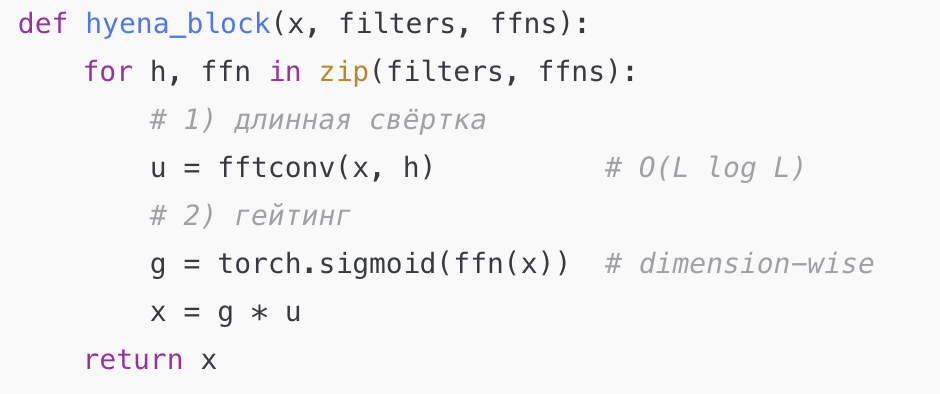
\includegraphics[scale=0.5]{pseudo.png}
    
\end{frame}

\begin{frame}{Результаты}
\begin{figure}
    \centering
    \begin{minipage}[t]{0.48\textwidth}
        \centering
        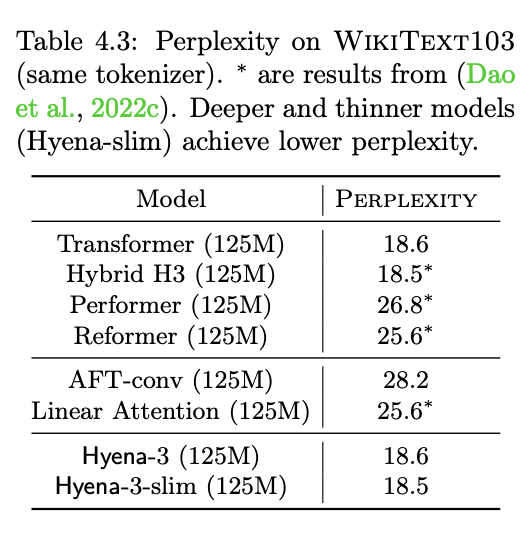
\includegraphics[width=\linewidth]{result1.png}
    \end{minipage}
    %\hfill
    \begin{minipage}[t]{0.48\textwidth}
        \centering
        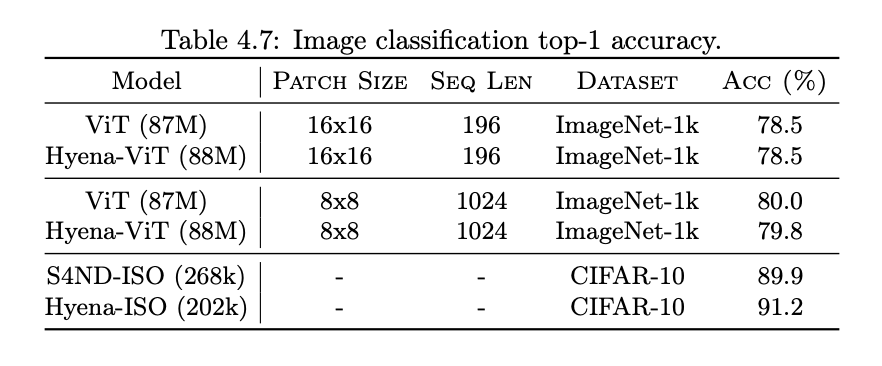
\includegraphics[width=\linewidth]{result2.png}
        
    \end{minipage}
\end{figure}
\end{frame}
	
\end{document}